%version 1.00,	date 12/05/2016	auteur(s) Pierre Porche
\speaker{\Juliana}

\begin{frame}
\frametitle{Développement Frontend}
\begin{block}{Technolgies Utilisées}
	\begin{itemize}
		\item Twig
		\item Bootstrap
		\item CSS
		\item jQuery
	\end{itemize}
\end{block}
\end{frame}

\begin{frame}
\frametitle{Développement Frontend}
\begin{block}{Twig: Le moteur de templates }
	\begin{itemize}
		\item Intégré directement dans le framework Symfony2
		\item Facilité de mise en place d'héritage de templates
		\item Idéal pour les Développeurs Frontend ou graphistes qui ne connaissent pas forcément le langage PHP et qui s'accommoderont parfaitement des instructions natives du moteur
	\end{itemize}
\end{block}
\end{frame}

\begin{frame}
\frametitle{Développement Frontend}
\begin{block}{ CSS et Bootstrap }
	\begin{itemize}
		\item Permettent de generer de vues responsives
		\item Très grande collection de composants
		\item Communauté qui propose des centaines d'autres composants
	\end{itemize}
\end{block}
\end{frame}

\begin{frame}
\frametitle{Responsive design}
	\begin{multicols}{2}
		\begin{figure}[!h]
			\begin{center}
				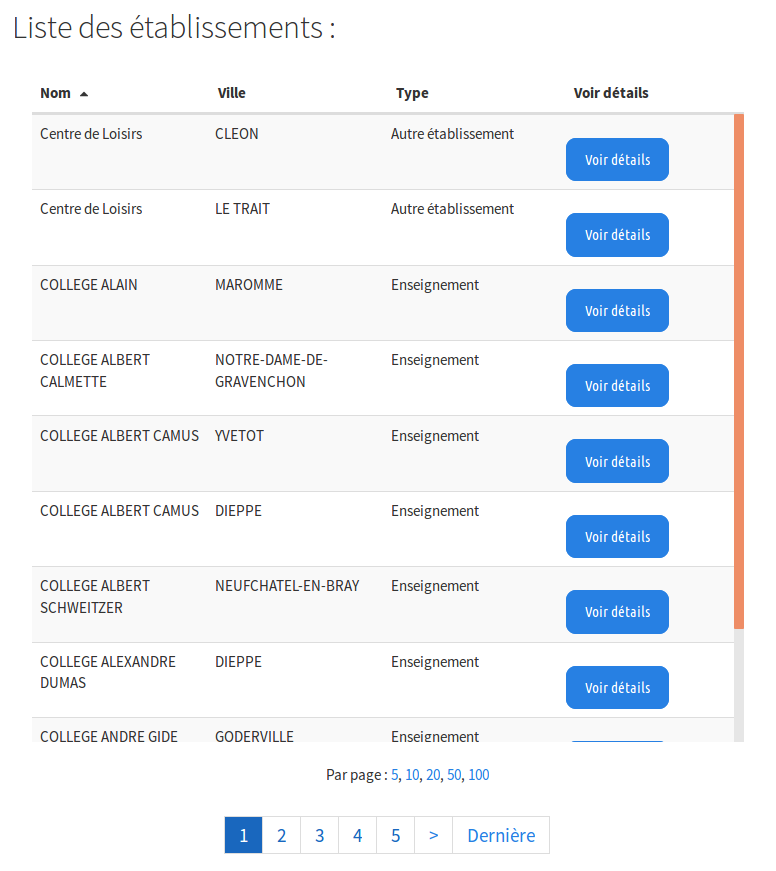
\includegraphics[scale=0.16]{images/screenshot1.png}

				\caption{Capture d'écran Accueil}
			\end{center}
		\end{figure}
		\begin{figure}[!h]
			\begin{center}
				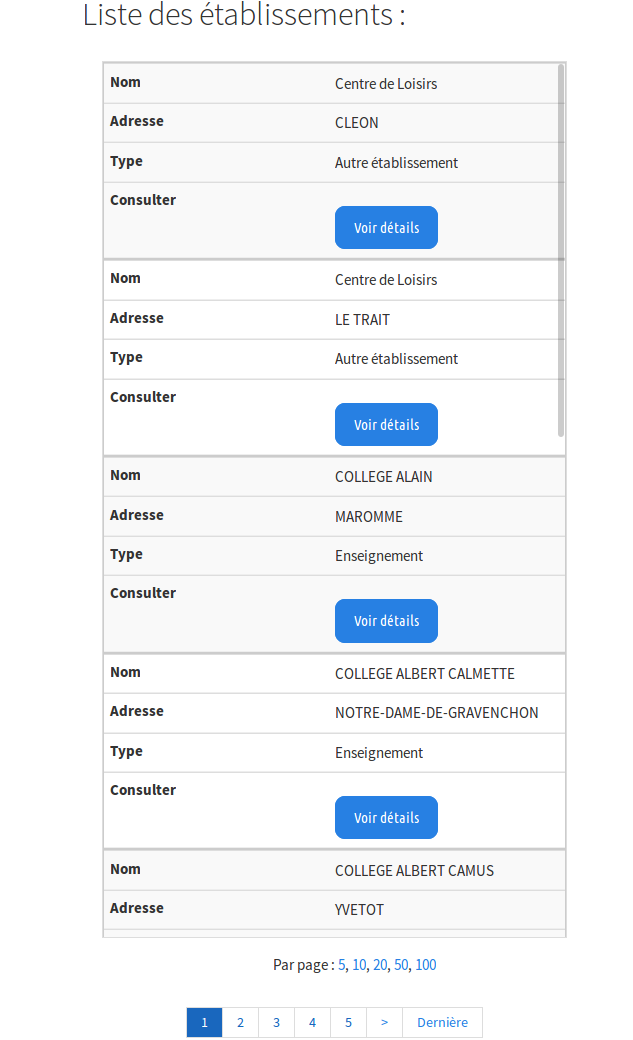
\includegraphics[scale=0.16]{images/screenshot2.png}
				\caption{Capture d'écran Accueil}
			\end{center}
		\end{figure}
	\end{multicols}

\end{frame}

